% -*- mode: LaTeX; tex-main-file: "../Notes.tex"; -*-
\section{Atomic Decompositions}
\label{sec:atomic}
\ifthenelse{\boolean{nofootnotes}}{\subsection{Time-Frequency Atoms}}
{\subsection{Time-Frequency Atoms\protect\footnotemark}
\footnotetext{Mallat~\cite{Mallat:1998} (p.67)}}
A linear time-frequency transform correlates the signal $x$ with a family of
waveforms that are well concentrated in time and in frequency.  These
waveforms are called \emph{time-frequency atoms}. Let us consider a general
family of time-frequency atoms  $\{\phi_{\gamma}\}_{\gamma \in \Gamma}$, 
where $\gamma$ might be a multi-index parameter.  We suppose that
$\phi_{\gamma} \in \LtwoR$ and that $\|\phi_{\gamma}\|=1$.  The
corresponding linear time-frequency transform of $x\in \LtwoR$ is defined
by  
%\begin{eqnarray*}
\begin{alignat}{2}
\T[x](\gamma)   &=\langle x,\phi_{\gamma} \rangle
                &&=\integral x(t)\phi^*_{\gamma}(t)\,dt \nonumber \\
\label{eqn:TFTF}&=\langle X,\Phi_{\gamma} \rangle
                &&=\integral X(\omega)\Phi^*_{\gamma}(\omega)\,d\omega 
\end{alignat}
The third equality holds by the Parseval formula (\ref{sec:Parseval}).

If $\phi_{\gamma}(t)$ is approximately zero when $t$ is outside a
neighborhood of an abscissa $u$, then  
$\langle x,\phi_{\gamma}\rangle$ 
depends only on the values of $x(t)$ in this neighborhood.  Similarly,
if  $\Phi_{\gamma}(\omega)$ is negligible for $\omega$ outside a
neighborhood of $\xi$, then~(\ref{eqn:TFTF}) shows that  
$\langle x,\phi_{\gamma} \rangle$ characterizes $X(\omega)$ in that
neighborhood. 

\renewcommand{\thedefine}{}
\begin{define}{\bf Energy Density. }
Suppose that for any point $(u,\xi)$ in the time-frequency plane there
exists a unique atom $\phi_{\gamma(u,\xi)}$ centered at this point.
The time-frequency support of  
$\phi_{\gamma(u,\xi)}$ 
specifies a neighborhood of $(u,\xi)$ where the energy of $x$ is
measured by 
\begin{align} \label{eqn:energy}
E_{\T[x]}(u,\xi) &=\left|\T[x](\gamma)\right|^2 \\
 &=\left|\langle x,\phi_{\gamma(u,\xi)}\rangle\right|^2 \nonumber
% &=\left|\integral x(t) \phi^*_{\gamma(u,\xi)}(t) \,dt\right|^2\nonumber
\end{align}
\end{define}
Later we will see that any such energy density is an averaging of the
\emph{Winger-Ville transform}, with a kernel that depends on the
atoms $\phi_{\gamma}$.

% (begin: inserted from windowedFT.tex)
\ifthenelse{\boolean{nofootnotes}}{\subsection{Windowed Fourier Transform}}
{\subsection{Windowed Fourier Transform\protect\footnotemark}
\footnotetext{Mallat~\cite{Mallat:1998} (p.69)}}
In 1946 Gabor~\cite{Gabor:1946} introduced windowed Fourier atoms to
measure the ``frequency variations'' of sounds.  A real and symmetric
window $g(t)=g(-t)$ is translated by $u$ and modulated by the
frequency $\xi$:
\[g_{u,\xi}(t) = e^{i2\pi\xi t}g(t-u)\]
The original window, $g$, has unit norm and therefore $\|g_{u,\xi}\|=1$
for any $(u,\xi)\in \R^2$.  The resulting windowed Fourier transform
of $x\in \LtwoR$ is 
\begin{eqnarray}\label{eqn:WindowedFT}
  \S[x](u,\xi) 
  &=& \langle x(t),g_{u,\xi} \rangle \nonumber\\
  &=& \integral x(t)g(t-u) e^{-i2\pi \xi t}\,dt
\end{eqnarray}
This transform is also called the \emph{short time Fourier transform}
because the multiplication by $g(t-u)$ localizes the Fourier integral
in the neighborhood of $t=u$.

As in~(\ref{eqn:energy}), one can define an energy density, called a
\emph{spectrogram}, by
\begin{align*}
  E_{\S[x]}(u,\xi)  &= \left|\S[x](u,\xi)\right|^2\\
  &= \left|\langle x(t),g_{u,\xi}\rangle\right|^2 
%  &= \left|\integral x(t) g(t-u) e^{-i2\pi\xi t}\,dt\right|^2\\
\end{align*}
The spectrogram measures the energy of $x$ in the time-frequency
neighborhood of $(u,\xi)$ specified by the Heisenberg box of
$g_{u,\xi}$. 
% (end: inserted from windowedFT.tex)

% (begin: inserted from wavelet.tex)
\ifthenelse{\boolean{nofootnotes}}{\subsection{Wavelet Transforms}}
{\subsection{Wavelet Transforms\protect\footnotemark}
\footnotetext{Mallat~\cite{Mallat:1998} (p.79)}}
\label{sec:atom-decomp}
To analyze signal structures of very different sizes, it is necessary
to use time frequency atoms with different time supports.  The wavelet
transform decomposes signals over dilated and translated wavelets.  A
wavelet is a function $\psi \in \LtwoR$ with zero average:
\[ \integral \psi(t)dt = 0\]
It is normalized, $\|\psi\|=1$ and centered in the neighborhood
$t=0$.  A family of time-frequency atoms is obtained by scaling $\psi$
by $s$ and translating it by $u$:
\[\psi_{u,s}(t) = \scale \psi \transcale\]
These atoms remain normalized: $\|\psi_{u,s}\|=1$.  The wavelet
transform of a function $x\in \LtwoR$ at time $u$ and scale $s$ is:
\begin{equation}
\label{eqn:wavelet}
\W[x](u,s) = \langle x,\psi_{u,s}\rangle
= \integral x(t)\scale \psi^* \transcale dt
\end{equation}

Like a windowed Fourier transform, a wavelet transform can measure the
time evolution of frequency transients.  This requires using a complex
analytic wavelet, which can separate amplitude and phase components.
An analytic wavelet can be used to measure \emph{instantaneous
frequencies}.  In contrast, real wavelets are often used to detect
sharp signal transitions.

\ifthenelse{\boolean{nofootnotes}}{\begin{define}{\bf Analytic Signals. }}
{\begin{define}{\bf Analytic Signals.\protect\footnotemark }
\footnotetext{Mallat~\cite{Mallat:1998} (p.84)}}
To analyze the time evolution of frequency tones, it is necessary to
use an analytic wavelet to separate the phase and amplitude
information of signals.
%\renewcommand{\thedefine}{}
%\begin{define}
%{\bf Analytic Signal. }
A function $x_a \in \LtwoR$ is said to be \emph{analytic} if its
Fourier transform is zero for negative frequencies:
\[X_a(\omega) = 0 \text{ if } \omega < 0.\]
\end{define}
An analytic function is necessarily complex but is entirely
characterized by its real part.  Indeed, the Fourier transform of its
real part $x = \Real[x_a]$ is 
\[X(\omega) = \frac{X_a(\omega) +
X^*_a(-\omega)}{2}\]
and this relation can be inverted to yield
\begin{equation}
\label{eqn:analFT}
X_a(\omega) = 
    \left\{ \begin{array}{lr}
        2X(\omega)& \text{ if } \omega \geq 0\\
        0 & \text{ if } \omega < 0
        \end{array} 
    \right.
\end{equation}
The analytic part $x_a(t)$ of a signal $x(t)$ is the inverse Fourier
transform of $X_a(\omega)$ defined by~(\ref{eqn:analFT}).

Equivalently, we obtain the analytic part of $x(t)$ a signal by
operating on the signal with the \emph{Hilbert transform}.  Precisely,
given a real signal $x(t)$, the analytic part is 
\[
x_a(t) = x(t) + i \H[x](t) = x(t) 
   + \frac{i}{\pi} \pv \integral \frac{x(s)}{t-s} ds
\]
where $\H$ denotes the Hilbert transform.  

\begin{define}{\bf Time-Frequency Resolution. }
% Mallat:1998} (p.85)
An analytic wavelet transform is calculated with an analytic wavelet
$\psi$ with the integral~(\ref{eqn:wavelet}). Its time-frequency
resolution depends on the time-frequency spread of the wavelet atoms  
$\psi_{u,s}$.  
\end{define} 
We suppose that $\psi$ is centered at 0, which implies that 
$\psi_{u,s}$ 
is centered at $t=u$.  
As shown in~\cite{Mallat:1998} (p.~85), the spread with respect to
time is $s^2 \sigma^2_t$, where $\sigma^2_t=\int t^2|\psi(t)|^2 dt$ is
the variance of $\psi$.  Since $\psi$ is analytic, 
$\Psi (\omega)$ 
is zero at negative frequencies, so the center frequency of
$\Psi $ is 
\[\eta =\int_0^{+\infty}\omega|\Psi (\omega)|^2 d\omega\]
The Fourier transform of $\psi_{u,s}$ is a dilation of $\Psi $ by
$1/s$:
\def\waveletFT{\Psi_{u,s}} 
\def\waveletFTomega{\Psi_{u,s}(\omega)} 
\[\waveletFTomega = \sqrt{s}\Psi (s\omega)e^{-i2\pi \omega
u}\]
Its center frequency is therefore $\eta/s$.  The energy spread of
$\waveletFT$ around $\eta/s$ is $\sigma^2_{\omega}/s^2$
(\cite{Mallat:1998} {\it ibid.}). 

Thus the energy spread of a wavelet time-frequency atom $\psi_{u,s}$
corresponds to a Heisenberg box centered at $(u, \eta/s)$, of size
$s\sigma_t$ along time and $\sigma_{\omega}/s$ along frequency.  The
area of the rectangle remains equal to $\sigma_t\sigma_{\omega}$ at
all scales, but the resolution in time and frequency depends on $s$.
As $s$ increases (resp.~decreases) frequency resolution increases
(resp.~decreases) while time resolution decreases (resp.~increases).
%as follows:\\ 
%\begin{center}
%\begin{tabular}{l|l|l}
%scale $s$ & increases & decreases\\
%\hline
%center frequency $\eta/s$ & decreases & increases \\
%frequency spread $\sigma_{\omega}/s$ & decreases & increases \\
%frequency resolution & improves & deteriorates \\
%time spread $s \sigma_t$ & increases & decreases \\
%time resolution & deteriorates &improves
%\end{tabular}
%\end{center}

An analytic wavelet transform defines a local time-frequency energy
density $E_{\W[x]}$, which measures the energy of $x$ in the Heisenberg box
of each wavelet $\psi_{u,s}$ centered at $(t, \xi)=(u, \eta/s)$:
\begin{equation}\label{eqn:energyDensity}
E_{\W[x]}(t,\xi) = \left|\W[x](u,s)\right|^2 =
\left|\W[x]\left(u,\frac{\eta}{\xi}\right)\right|^2
\end{equation}
This energy density is called a \emph{scalogram}.
% (end: inserted from wavelet.tex)

% (begin: inserted from instantfreq.tex)
\ifthenelse{\boolean{nofootnotes}}{\subsection{Instantaneous Frequency}}
{\subsection{Instantaneous Frequency\protect\footnotemark}
\footnotetext{Mallat~\cite{Mallat:1998} (p.91)}}
\label{sec:instfreq}
A cosine modulation 
\[
x(t) = a(t) \cos(\omega_0 t + \phi_0) 
= a(t) \cos\phi(t), \quad \text{ for } a(t) \geq 0
\]
has a frequency $\omega_0$ that is the derivative of the phase
$\phi(t) = \omega_0 t + \phi_0$.  The {\it instantaneous frequency} is
defined as a positive derivative of the phase:
\begin{equation}
\label{eqn:instfreq}
\omega(t) = \phi'(t) \geq 0.
\end{equation}
By adapting the sign of $\phi(t),$ the derivative can be taken to be
positive.  Since there are many possible choices of $a(t)$ and
$\phi(t),$ it is clear that $\omega(t)$ is not uniquely defined
relative to $x$. 

Recall that 
%\begin{define}{\bf Analytic Signal} (\cite{Mallat:1998} p.~84)
a function $x_a \in \LtwoR$ is said to be \emph{analytic} if its
Fourier transform is zero for negative frequencies:
\[X_a(\omega) = 0 \text{ if } \omega < 0.\]
%\end{define}
%\end{definition}
An analytic function is necessarily complex but is entirely
characterized by its real part, $x = \Real[x_a]$, which has the
Fourier transform
\[X(\omega) = \frac{X_a(\omega) +
X^*_a(-\omega)}{2}\]
and this relation can be inverted to yield
\begin{equation}%\label{eqn:analFT}
X_a(\omega) = 
    \left\{ \begin{array}{ll}
        2 X(\omega),& \quad \text{ if } \omega \geq 0\\
        0, & \quad \text{ if } \omega < 0
        \end{array} 
    \right.
\end{equation}
The analytic part $x_a(t)$ of a signal $x(t)$ is the inverse Fourier
transform of $X_a(\omega)$ defined by~(\ref{eqn:analFT}).
Writing the analytic part of $x$ as the modulus times the complex
exponential,
\[x_a(t) = a(t)\exp[i\phi(t)] = a(t)[\cos\phi(t) + i \sin\phi(t)]\]
it is clear that 
\[x(t) = \Real[x_a] = a(t)\cos\phi(t)\]
The factor $a(t)$ is the \emph{analytic} amplitude of $x(t),$ while
$\phi'(t)$ is the instantaneous frequency.  Both $a(t)$ and $\phi'(t)$
are uniquely defined. 

% Mallat:1998 (p.92)
\begin{example}\protect\footnotemark
\footnotetext{Mallat~\cite{Mallat:1998} (p.92)}
If $x(t) = a(t)\cos(\omega_0 t + \phi_0)$, then 
\begin{equation}\label{eqn:CosineFT} 
X(\omega)=
\frac{1}{2}\left(\hat{a}(\omega - \omega_0) e^{i \phi_0} + 
\hat{a}(\omega + \omega_0) e^{-i \phi_0} \right)
\end{equation}
where $\hat{a}(\omega)$ denotes the \FT\ of $a(t)$.
If the variations of $a(t)$ are slow compared to the period $T =
2\pi/\omega$, which is achieved by requiring that the support of
$\hat{a}$ be included in $[-\omega_0,\omega_0]$, then the second term
on the right of~(\ref{eqn:CosineFT}) is zero for $\omega>0$ and 
\[X_a(t) = \hat{a}(\omega - \omega_0) e^{i \phi_0}\]
by~(\ref{eqn:analFT}).  So $x_a(t) = a(t)\exp[i(\omega_0t+\phi_0)]$.
\end{example}

\begin{example} If a signal $x$ is the sum of two sinusoidal waves, 
$a\cos(\omega_1t) + a\cos(\omega_2t)$, then 
\begin{eqnarray*}
x_a(t)&=&a e^{i \omega_1t} + a e^{i \omega_2t}\\
&=& a\cos[ (\omega_1-\omega_2)t/2]\exp[i (\omega_1+\omega_2)t/2]
\end{eqnarray*}
The instantaneous frequency is $\phi'(t)=(\omega_1+\omega_2)/2$ and
the amplitude is 
\[
a(t)= a \left|\cos[ (\omega_1-\omega_2)t/2]\right|
\]
This result is not satisfying because it does not reveal that the
signal includes two sinusoidal waves of the same amplitude.  It
measures an average frequency value.  The next sections explain how to
measure the instantaneous frequencies of several spectral components
by separating them with a windowed Fourier transform or a wavelet
transform. 
\end{example}
% (end: inserted from instantfreq.tex)

% (begin: inserted from ridges.tex)
\ifthenelse{\boolean{nofootnotes}}{\subsection{Fourier Ridges}}
{\subsection{Fourier Ridges\protect\footnotemark}
\footnotetext{Mallat~\cite{Mallat:1998} (p.94)}}
% Mallat:1998 (p.94)
The spectrogram $E_{\S[x]}(u,\xi)$ measures the energy of $x$ in a
time-frequency neighborhood of $(u,\xi)$.  The ridge algorithm
computes the instantaneous frequencies from the local maxima of
$E_{\S[x]}(u,\xi)$.  This approach was introduced by Delprat, Escudi\'{e},
Guillemain, Kronland-Martinet, Tchamitchian and
Torr\'{e}sani~\cite{Delprat:1992} to analyze musical sounds.  Since
then, it has found applications for a wide range of signals that have
time varying frequency tones.

% Mallat:1998 (p. 98)
When the signal contains several spectral lines \emph{whose
frequencies are sufficiently apart}, the windowed Fourier transform
separates each of these components and the ridges detect the evolution
in time of each spectral component.
%\footnote{Mallat~\cite{Mallat:1998} (p.98)}

%% (begin: included from icassp file windowedFT.tex)
The windowed Fourier transform is computed with a symmetric window
$g(t)=g(-t)$ with support $t\in[-1/2,1/2]$ and unit norm, $\|g\|=1$.  
For a fixed scale $s$, $g_s(t)=s^{-1/2}g(t/s)$ has a support of size
$s$ and unit norm.  The corresponding windowed Fourier atoms are 
$g_{s,u,\xi}(t)=g_s(t-u)e^{i \xi t}$
and the windowed Fourier transform is defined by 
\[
\S[x](u,\xi) =\integral x(t)g_s(t-u)\e^{-i \xi t}dt
\]

If $x(t)=a(t)cos\phi(t)$, then the transform $\S[x](u,\xi)$
has the following relation to the instantaneous frequency of $x$:
\begin{equation}
\label{eqn:freqest}
\S[x](u,\xi)=\frac{\sqrt{s}}{2}a(u)\exp(i[\phi(u)-\xi u])
            \left(\hat{g}(s[\xi-\phi'(u)])+\epsilon\right)%\epsilon_{u,\xi}\right)
\end{equation}
for all $\xi \geq 0$.  For bounds on $\epsilon$,
see Mallat~\cite{Mallat:1998}.  Delprat \emph{et al.} \cite{Delprat:1992}
prove a similar result for Gaussian $g$.

If we can neglect the corrective term ($\epsilon$) %$\epsilon_{u,\xi}$,
then~(\ref{eqn:freqest}) enables us to measure $a(u)$ and $\phi'(u)$
using $\S[x](u,\xi)$.  Briefly, the corrective term is negligible when two
conditions are satisfied.
First, let the bandwidth of $\hat{g}$ be $\Delta \omega$ such that 
$|\hat{g}(\omega)|\ll 1$ when $|\omega| \geq \Delta \omega$. 
Then we require that 
\[
\phi'(u) \geq \frac{\Delta \omega}{s}
\]
The second condition permitting us to neglect $\epsilon$ %$\epsilon_{u,\xi}$ 
is
that $a(t)$ and $\phi'(t)$ must have small relative variations over the
support of the scaled window $g_s$.  
If these two conditions are met, then~(\ref{eqn:freqest}) shows that
for each $u$, the spectrogram $\left|\S[x](u,\xi)\right|^2$ is maximized at
$\xi(u)=\phi'(u)$.  The corresponding time-frequency pairs
$(u,\xi(u))$ are called \emph{ridge points}.  
Such points indicate that the predominant spectral components of the
signal occur at frequencies $\phi'(u)=\xi(u)$ with analytic
amplitudes, computed from~(\ref{eqn:freqest}), 
\[
a(u) = \frac{2\left|\S[x](u,\xi(u)\right|}{\sqrt{s}|\hat{g}(0)|}
\]

% Mallat:1998 (p. 98)
When the signal contains several spectral lines \emph{whose
frequencies are sufficiently apart}, the windowed Fourier transform
separates each of these components and the ridges detect the evolution
in time of each spectral component.  Suppose, for instance, that $x$
has the form 
\[
x(t) = a_1(t)\cos\phi_1(t) + a_2(t)\cos\phi_2(t)
\]
where $a_k(t)$ and $\phi'_k(t)$ have small variations over intervals
of size $s$ and $s\phi'_k(t)\geq\Delta\omega$.  Since the Fourier
transform is a linear operation, equation~(\ref{eqn:freqest}) implies
that 
%\begin{eqnarray}
\begin{equation}
\label{eqn:2ridges}
\S[x](u,\xi)\approx\frac{\sqrt{s}}{2}
a_1(u)\exp(i[\phi_1(u)-\xi u])\hat{g}(s[\xi-\phi_1'(u)])%\nonumber \\
\end{equation}
\[+\frac{\sqrt{s}}{2}
a_2(u)\exp(i[\phi_2(u)-\xi u])\hat{g}(s[\xi-\phi_2'(u)])\]
%\end{eqnarray}
The two spectral components can be discriminated if for all $u$,
$\hat{g}(s|\phi'_1(u)-\phi'_2(u)|) \ll 1$
%\[\hat{g}(s|\phi'_1(u)-\phi'_2(u)|) \ll 1\]
which means that the frequency difference is larger than the bandwidth
of $\hat{g}(s\omega)$:
\begin{equation}
\label{eqn:cond}
|\phi'_1(u)-\phi'_2(u)|\geq \frac{\Delta \omega}{s}
\end{equation}
In this case, when $\xi = \phi'_1(u)$, the second term
of~(\ref{eqn:2ridges}) can be neglected and the first term generates a
ridge point from which we may recover $\phi'_1(u)$ and $a_1(u)$.
Similarly for the case $\xi = \phi'_2(u)$.  The ridge points are
distributed along two time-frequency lines $\xi(u)=\phi'_1(u)$ and 
$\xi(u)=\phi'_2(u)$.  This result is valid for any number of
time-varying spectral components, as long as the distance between any
two instantaneous frequencies satisfies~(\ref{eqn:cond}).  For those
values of $u$ at which the spectral lines are too close, they
interfere and destroy the ridge pattern.

\begin{center}
\begin{figure}
\ifthenelse{\boolean{nofigures}}{}{
%	\pdfimage
%        width 120 mm 
%        height 70 mm
\centering
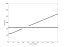
\includegraphics[width=120mm, height=70mm]{\HOME/figures/PureLin440Ridges}
}
\caption{The local maximum moduli of the spectrogram are the ridge
points that locate instantaneous frequencies.}
\label{fig:ridges}
\end{figure}
\end{center}
%% (end: included from icassp file windowedFT.tex)

Figure~\ref{fig:ridges} displays the ridges computed from the local
maxima of the spectrogram of
\begin{equation}
\label{eqn:purelin440}
x(t) = 0.5\cos(2\pi440t) + 0.4\cos(2\pi\alpha440t)
\end{equation}
where $\alpha = 0.5 + 1.5t$.  That is, the first summand is a pure 440 
Hz tone with a constant amplitude of 0.5, while the second term 
has amplitude 0.4 and a frequency that increases linearly from 220 Hz
to 880 Hz over the interval $t\in [0,1]$.  The ridges fail to
accurately describe the frequency content of the signal when $t$
ranges from about 0.3 to 0.4 seconds.  Here the instantaneous
frequencies are too close and the frequency resolution is not
sufficient to distinguish them.

\ifthenelse{\boolean{nofootnotes}}{\begin{define}{\bf Wavelet Ridges. }}
{\begin{define}{\bf Wavelet Ridges.\protect\footnotemark }
\footnotetext{Mallat~\cite{Mallat:1998} (p.102)}}
Windowed Fourier atoms have a fixed scale and thus cannot follow
the instantaneous frequencies of rapidly varying events such as
hyperbolic chirps.  In contrast analytic wavelet transform modifies
the scale of its time-frequency atoms.  The ridge algorithm of Delprat
{\it et al} ({\it op.~cit.}) can be extended to analytic wavelet
transforms to accurately measure frequency tones that are rapidly
changing at high frequencies.
\end{define}
% (end: inserted from ridges.tex)

\subsection{Matching Pursuit}
%\ifthenelse{\boolean{nofootnotes}}{\subsection{Matching Pursuits}}
%{\subsection{Matching Pursuits\protect\footnotemark}
%\footnotetext{Gribonval, {\it et~al}~\cite{Gribonval:1996}}}
\label{sec:MP}
A \emph{matching pursuit}~\cite{Mallat:1993} is an iterative algorithm
that decomposes the signal over \emph{dictionary} vectors.
A dictionary is a family of vectors 
$\mathcal{D}= \{g_\gamma\}_{\gamma\in\Gamma}$ 
included in a Hilbert space $\Hilbert$, with a unit norm
$\|g_\gamma\|=1$.  Such a family can be constructed by scaling,
translating and modulating a single window function $g(t) \in \LtwoR$.
We suppose that $g(t)$ is real, continuously differentiable and
$O(\frac{1}{t^2+1})$.  We further impose that $\|g\|=1$, that the
integral of $g(t)$ is non-zero, and that $g(0)\neq 0$.  
For any scale $s$, translation $u$, and frequency modulation $\xi$, we
denote $\gamma = (u,s,\xi)$ and define
\begin{equation}\label{eq:ggamma}
g_\gamma(t) 
= \frac{1}{\sqrt{s}}g\left(\frac{t-u}{s}\right) e^{i2\pi\xi t}
\end{equation}
The index $\gamma$ is an element of the set 
$\mathbf{\Gamma} = \Real \times \Real^+ \times \Real$.  The factor
$1/\sqrt{s}$ normalizes the norm of $g_\gamma$ to 1. If $g(t)$ is
even, which is generally the case, $g_\gamma(t)$ is centered at the
abscissa $u$.  Its energy is mostly concentrated in a neighborhood of
$u$, whose size is proportional to $s$.  Let $\hat{g}(\omega)$ be the
\FT\ of $g(t)$.  Equation~(\ref{eq:ggamma}) yields
\[
\hat{g}_\gamma(\omega) 
= \sqrt{s}\hat{g}(s(\omega - \xi))e^{-i2\pi(\omega-\xi)u}
\]

The matching pursuit algorithm iteratively decomposes a signal over
dictionary vectors as follows.
Let $R^0x(t)=x(t)$, and suppose that we have computed the $n^{th}$
order \emph{residue}, $R^nx$, for $n\geq 0$.  We then choose an
element, $g_{\gamma_n}$ which closely ``matches'' the residue in the
following sense:
\[
|C(R^nx,g_{\gamma_n})| = \sup_{\gamma \in \Gamma} |C(R^nx,g_\gamma)|
\]
where $C(x,g_\gamma)$ is a correlation function which measures the
similarity between $x$ and $g_\gamma$.  An example is the usual inner
product, $\langle x,g_\gamma \rangle$.

Next, decompose the residue as 
\[
R^nx(t) = C(R^nx,g_{\gamma_n})g_{\gamma_n}(t) + C(R^{n+1}x(t)
\]
which defines the residue for step $n+1$, and fully specifies the
algorithm recursion.  

With the usual inner product as the correlation function, it can be
shown (\cite{Mallat:1998}, p.422) that the magnitude of the residue,
$\|R^nx\|$ converges to 0 exponentially as $n$ increases.  This yields
the following atomic signal decomposition:
\begin{equation}\label{eq:MP}
x(t) = \sum_{n=0}^\infty C(R^nx,g_{\gamma_n})g_{\gamma_n}(t) 
\end{equation}


